This chapter will describe the mission system and the creation of custom content as these are closely tied.
From the requirements listed in Section \ref{gamedesign:selectionofgametype:importantstuff}, custom content creation will contribute towards satisfying requirement 3, and the mission system contributes toward requirements 1, 2, 4, 5 and 6.

\section{Mission System}
The mission system is the system that handles the missions, maps and waves of enemies.
It supports custom created content, which will be described in Section \ref{sec:modules:missions:customcontent}.
A single mission contains several waves of enemies, each started when all the players declare themselves as ready.
Waves spawn enemies from a series of spawn points at a certain rate, in the attempt to populate the map with enemies according to defined boundaries.
Furthermore, waves have a probability on every tick to create an objective that the players can complete to earn a higher score.

\section{Custom Content}\label{sec:modules:missions:customcontent}
The game design declare that the game should supports custom content, described in Section \ref{sec:selectionofgametype:customcontent}.
Custom content must be placed in the \lstinline|Application.persistentDataPath| directory, and consists of several files.
The main file is a JSON formated text-file, specifying the content that can be seen in figure \ref{fig:json_chart}.
To encapsulate the desired data, many formats could have been used successfully.
The choice fell upon JSON due to it being an open, human readable format that can be easily edited using regular text editors.

\begin{figure}[H]
    \centering
    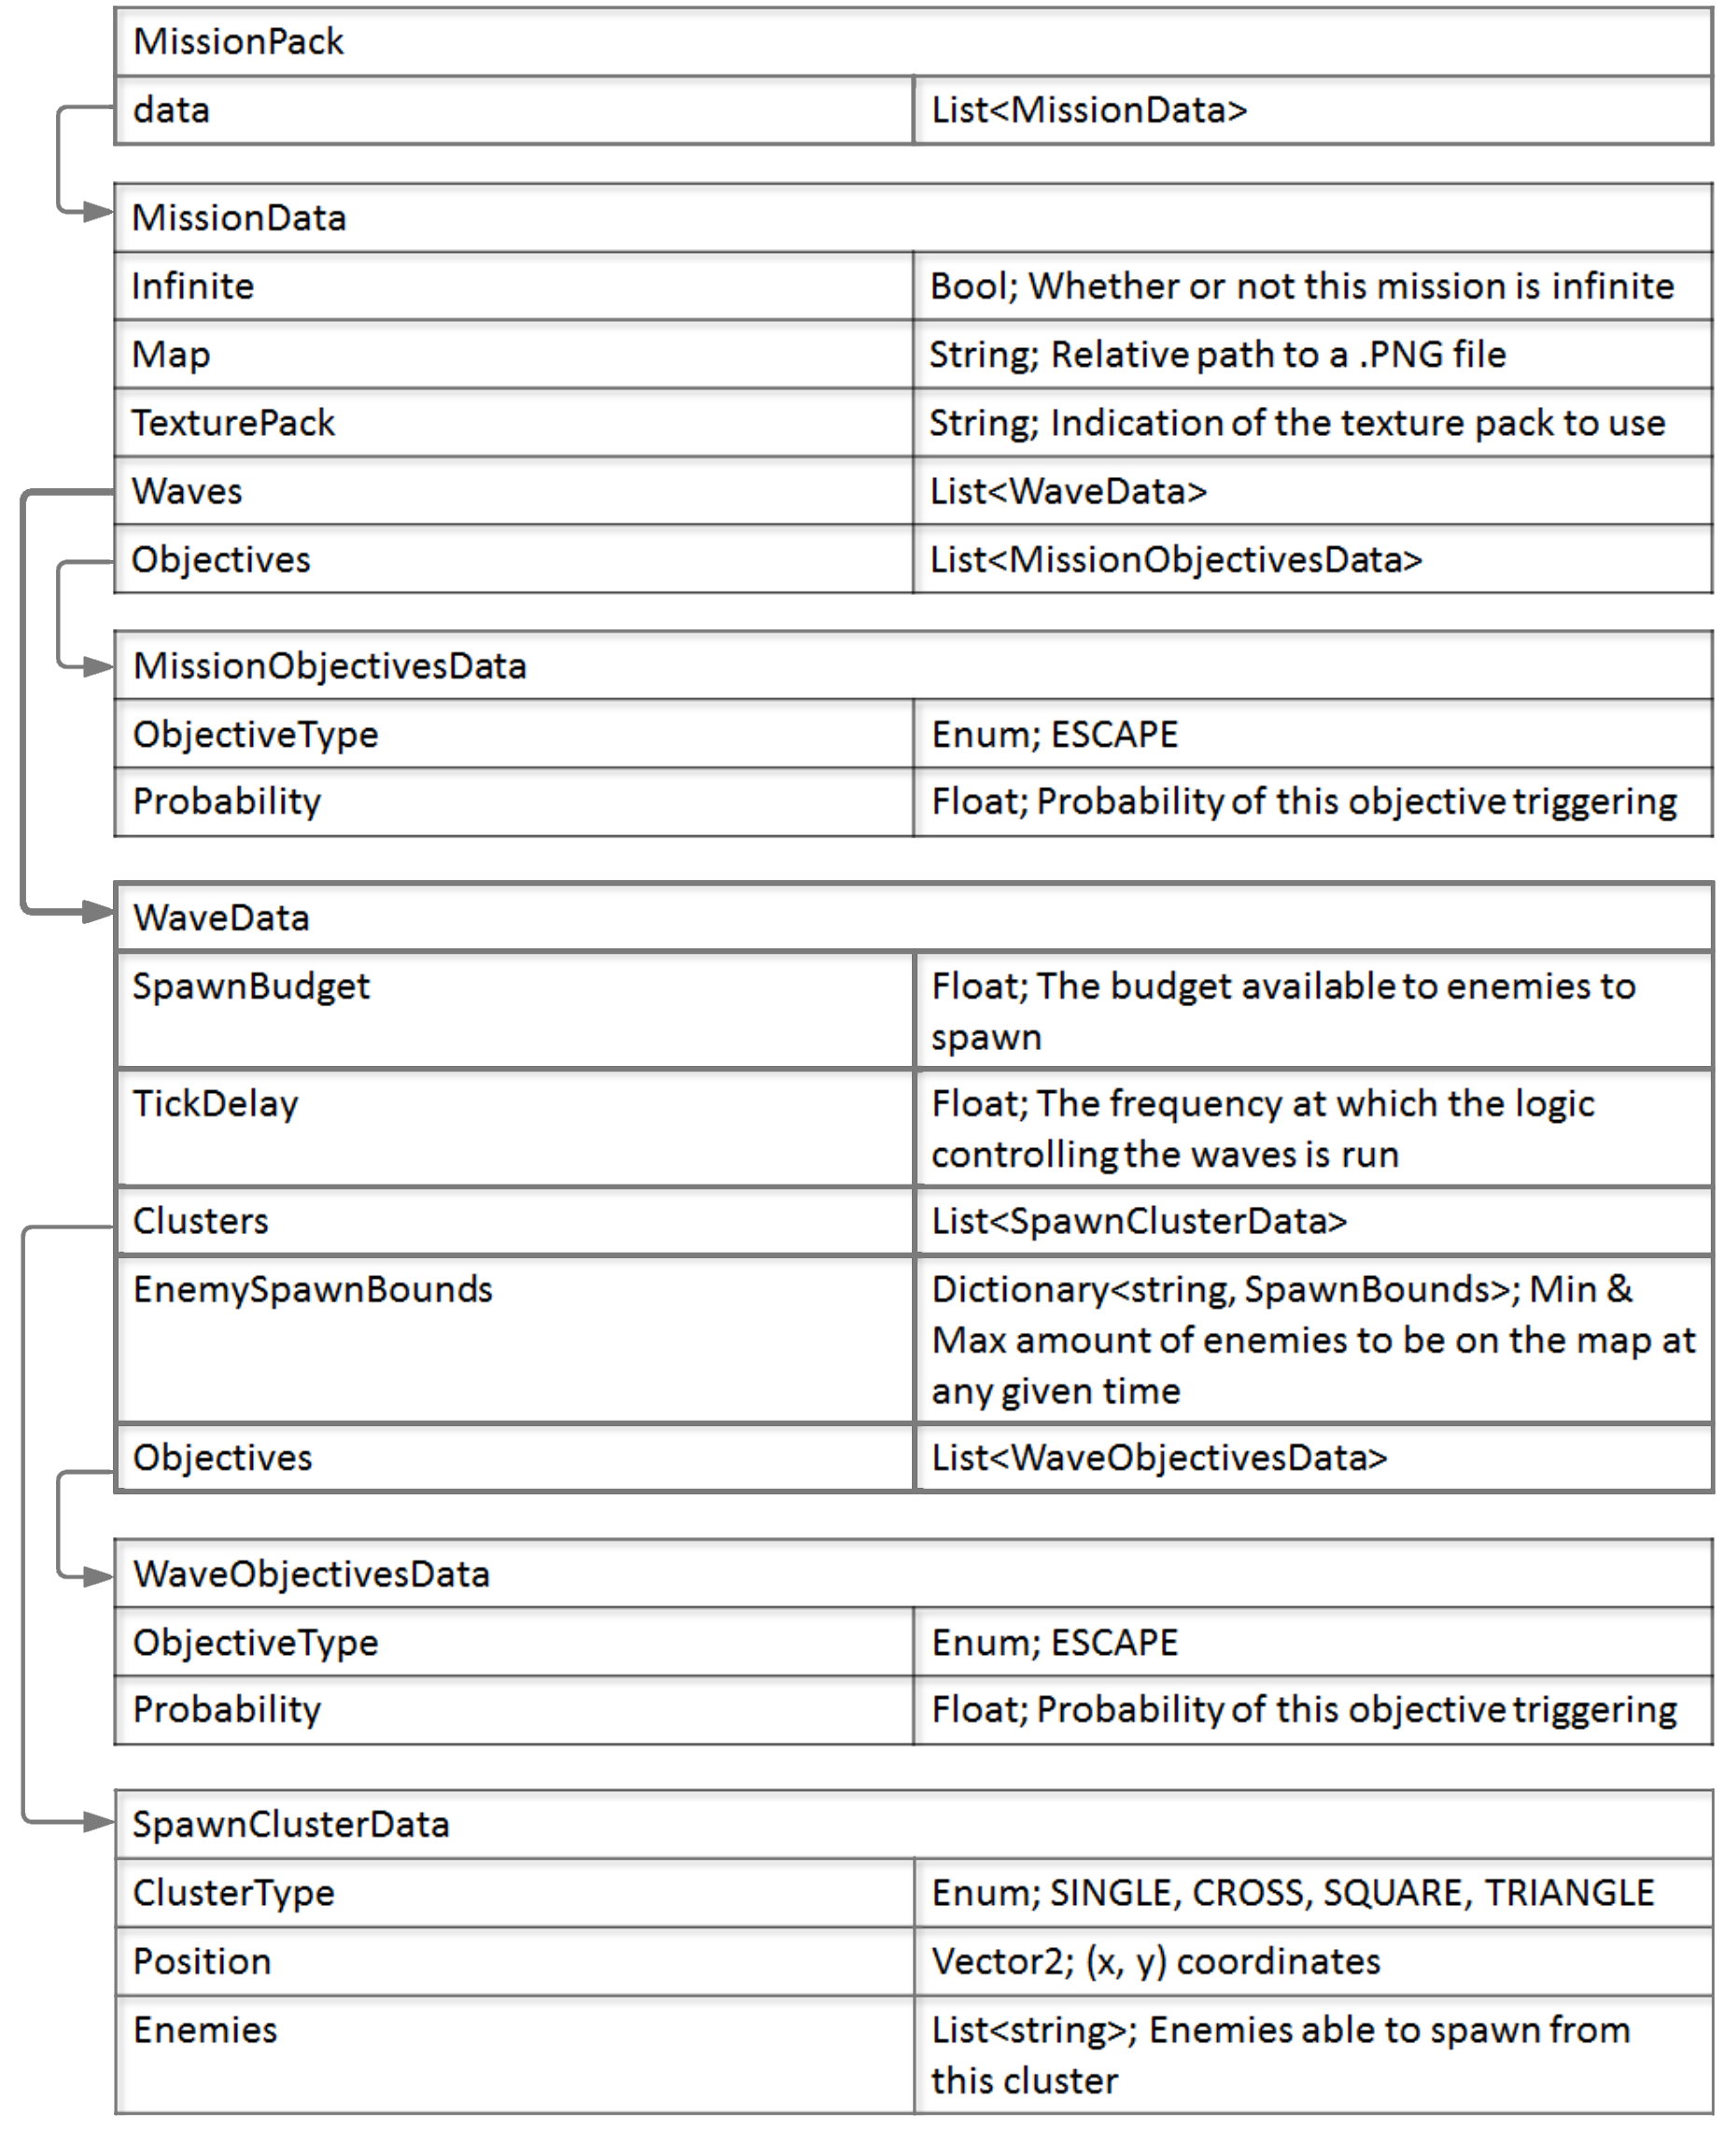
\includegraphics[width=1\textwidth]{figures/missions/chart.png}
    \caption{Chart depicting data contained in JSON file for content creation.}
    \label{fig:json_chart}
\end{figure}

As seen in figure \ref{fig:json_chart}, for the custom map we use the PNG (Portable Network Graphics) format.
The choice of PNG was for the following reasons:
\begin{itemize}
    \item The PNG format is ubiquitous, in that there exists support for it almost anywhere, including in Unity3d - both in terms of API and the editor itself.
    \item It being ubiquitous means that we do not have to develop additional software in order to edit maps - most mainstream image editors support the PNG format.
    \item The PNG allows us to encode \textit{enough} information. 
    	\textit{Enough} being relative, but each colorchannel for each individual pixel offers 1 \texttt{byte} of information.
    	With each pixel being encoded with RGBA (red, green, blue and alpha) channels that gives us a total of 4 \texttt{bytes} of information, for each pixel.
\end{itemize}

A sample map can be seen in figure \ref{fig:png_map}.
